% fixture: tikz/node-text
% tier: T3
% engine: document
% specials: compare
% covers: node text in lines (align= without a text width: \\ and \\[skip], an empty line, flush and justified alignments, a font option's baselines), in a minipage of a text width (each text action's skips, \spaceskip and \xspaceskip, \\ as \@centercr and in justified text, a text color in the paragraph, an empty text), node font= (the node's em for its inner sep and shifts), in the first paragraph after a heading (\clubpenalty 10000)
% issue: #326
\documentclass{article}
\usepackage{tikz}
\usetikzlibrary{positioning}
\begin{document}
\section{Nodes}
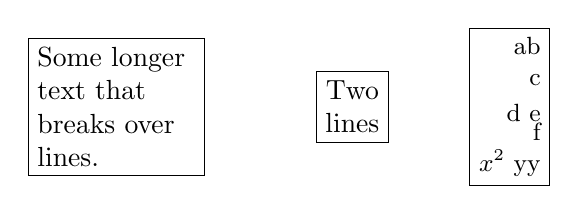
\begin{tikzpicture}[every node/.style={draw}]
  \node[text width=2cm] at (0,0) {Some longer text that breaks over lines.};
  \node[align=center] at (3,0) {Two\\lines};
  \node[align=right,font=\small] at (5,0) {ab \\ c\\[2pt] d e\\[-1ex] f \\ $x^2$ yy};
\end{tikzpicture}

Text widths:
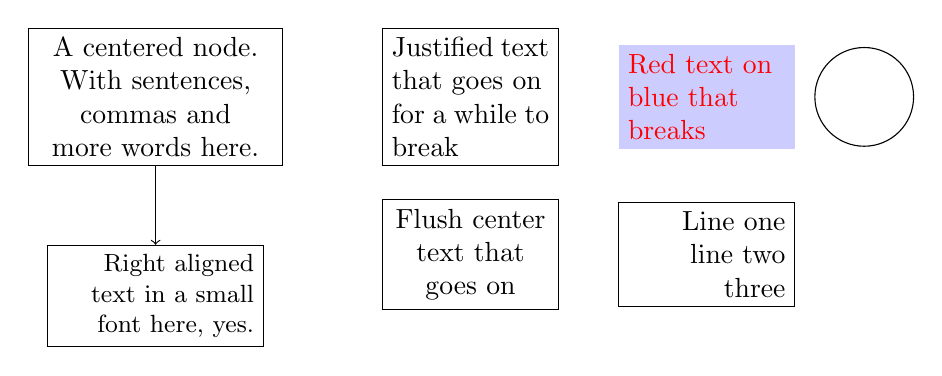
\begin{tikzpicture}
  \node[draw,text width=3cm,align=center] (a) {A centered node. With sentences, commas and more words here.};
  \node[draw,text width=25mm,align=right,font=\small,below=of a] (b) {Right aligned text in a small font here, yes.};
  \node[draw,text width=2cm,align=justify] at (4,0) {Justified text that goes on\\ for a while to break};
  \node[draw,text width=2cm,align=flush center] at (4,-2) {Flush center text that goes on};
  \node[fill=blue!20,text=red,text width=2cm,align=flush left] at (7,0) {Red text on blue that breaks~};
  \node[draw,text width=2cm,align=flush right] at (7,-2) {Line one \\ line two\\three};
  \node[draw,text width=1cm,circle] at (9,0) {};
  \draw[->] (a) -- (b);
\end{tikzpicture}
and fonts:
\tikz[baseline] \node[node font=\footnotesize,draw,inner sep=.5em,align=flush center] {x\\[1ex]yy\\};
\tikz \node[node font=\small\bfseries,font=\itshape,text width=4em,draw] {Text in a small bold font};
\end{document}
